\documentclass[conference]{IEEEtran}
\usepackage[T1]{fontenc}
\usepackage{times}
\usepackage[numbers]{natbib}
\usepackage{graphicx}
\pagestyle{empty}
\begin{document}
\title{When Should a Mobile Robot Ask a Peer for Another View?}
\author{Author names omitted for anonymous review}
\maketitle
\thispagestyle{empty}
\begin{abstract}
When a tracked robot loses sight of a docking target, should it turn its own camera or ask a wheeled manipulator to look? We compared these choices on identical simulated starts and scored the recipient's terminal pose. In 24 open-room scenes, requesting help when the initial target pose was missing completed every dock with 13 requests. Three seconds of active local search also completed every dock with zero requests. An opaque screen changed the value of the peer's viewpoint. On 16 held-out starts, local search alone completed eight docks. A learned request rule completed all 16 with 14 requests. Searching locally first and requesting only after a miss completed the same 16 with eight requests, taking 0.33\,s longer per attempt on average. In a further 16 scenes with a common six-second sensing deadline and variable helper offers, adaptive selection and fixed local-first search succeeded on the same 13 starts with six requests each. Local-only search succeeded eight times, while requesting immediately succeeded twelve times with twelve calls. In this task a timely peer measurement rescued otherwise unsuccessful docks, while learning the request rule yielded little additional utility over an active local-first baseline. Physical endpoints remain unmeasured.
\end{abstract}
\IEEEpeerreviewmaketitle

\section{Choosing between two ways to see}
Suppose a robot turns toward a known wall, but its first camera frame contains no docking target. A second robot can point its own camera at that wall and transmit a metric waypoint. A successful dock after the exchange admits several explanations. The recipient may have reached the target using a previously known location. Turning its own camera may have been enough. Finally, it may genuinely have needed the peer's viewpoint. These alternatives give different predictions when we change the reported waypoint or the recipient's sensing budget.

Our experiment holds the vehicles, terminal criterion and controller fixed while changing who looks and which message reaches the controller. We also compare a visibility rule with a fixed-budget random assignment. These comparisons answer distinct questions. The first concerns a message's causal effect on a task. The second concerns the ability to allocate calls on a particular set of scenes. A third comparison gives the recipient an active sensing action at the same time budget as the donor.

\subsection{Related work}
KnowNo calibrates when a language-model planner needs human clarification \cite{ren}. Fleet-DAgger allocates scarce human supervision across robots \cite{hoque}. Proactive collaboration has already demonstrated that embodied agents can recruit heterogeneous teammates \cite{recruitment}. Physical viewpoint assistance has used a moving camera to recover object shape for manipulation \cite{viewpoint}. When2com learns communication groups, and V2V4Real compares collaborative perception across vehicles and synchronization conditions \cite{liu,xu}. Marcotte et al. estimate the value of a message by forward-simulating a teammate with and without it \cite{marcotte}. We measure that difference in a tracked recipient's terminal docking task. An inexpensive active local sensing action provides a comparator to the peer's observation.

Communication actions in multi-agent POMDPs explicitly trade information against coordination cost~\cite{askpomdp}. Uncertainty-aware policy steering distinguishes ambiguity about the instruction from the feasibility of sampled actions~\cite{ups}. We test a narrower engineering question. Under a common simulated sensing deadline, can a short history of failed detections and a quoted helper service change which action maximizes realized docking utility?

\section{An actionable observation in a shared world}
A tracked base and a wheeled manipulator occupy one MuJoCo world. A fixed wall heading and a surveyed start pad define the task frame. We vary the board position in the plane near the wall and the tracked robot's starting heading. The initial camera can face away from the board. Six engineering scenes preceded the fixed set of 24 evaluation seeds. Both sets use the same three room presets. The seeds define different starts within those presets.

The recipient first inspects its own RGB frame. An OpenCV detector identifies a known 180\,mm square fiducial and estimates its metric pose. When requested, the manipulator points its camera toward the board at a fixed observation pose. The message contains an estimated waypoint, frame, simulation timestamp and source image identity. The recipient steers using the waypoint, known mounting geometry and odometry integrated from ideal body velocity measurements. Its actuator path has no access to the true target or base pose. A separate physics verifier reads those states. Docking requires position error below 8\,cm, absolute yaw error below 0.15\,rad and a stable stop for 0.5\,s. Calibration, odometry drift, image noise and arbitrary target-facing headings remain open transfer questions.

\begin{figure}[t]
\centering
\begin{tabular}{@{}cc@{}}
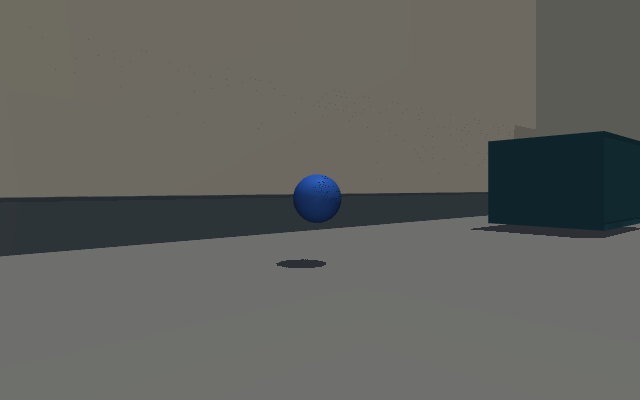
\includegraphics[width=.47\columnwidth]{figures/recipient-before.png}&
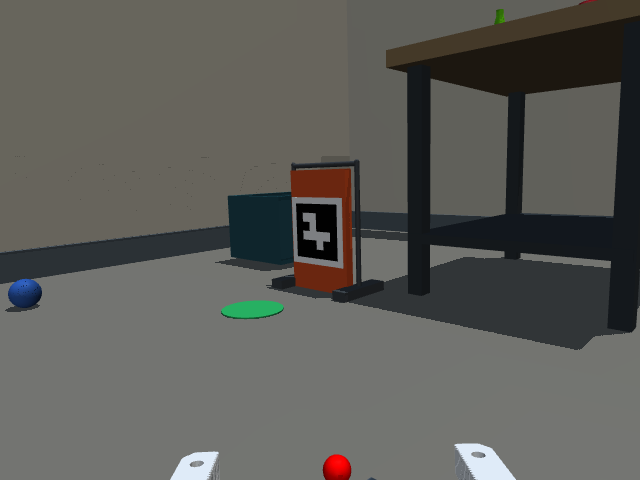
\includegraphics[width=.47\columnwidth]{figures/donor-observation.png}\\
(a) Initial recipient view & (b) Helper observation
\end{tabular}
\caption{Actual policy inputs from evaluation scene 848000. The tracked robot's initial frame did not yield a target pose. The donor's measured waypoint drove 160 commands and the recipient stopped 2.37\,cm from the scoring position. A replay reproduced the command hash and terminal error.}
\end{figure}

\subsection{Paired interventions}
We save the initial state, local frame and request decision before branching. For the three donor-packet conditions we restore the same state after the donor has looked. One branch receives the correct measurement, one receives a report older than the 0.75\,s freshness limit, and one receives the report from the next scene in a fixed cyclic permutation. A fixed visibility rule calls whenever the initial local detector fails. A random policy makes exactly the same number of calls using a preassigned seed ordering. For the active comparator, the recipient can rotate toward the surveyed wall and attempt detection repeatedly for up to three seconds. It then uses the same docking controller. Immediate failures from missing or expired packets count as failures.

\begin{table}[t]
\centering\caption{Matched docking outcomes in 24 simulated scenes.}
\begin{tabular}{lrr}\hline
Policy or packet condition & Docks & Peer calls \\\hline
Local initial frame & 11 & 0 \\
Local active search & 24 & 0 \\
Always request & 24 & 24 \\
Request on missing pose & 24 & 13 \\
Random allocation, matched count & 16 & 13 \\
Expired packet & 0 & 24 \\
Packet from another scene & 4 & 24 \\\hline
\end{tabular}
\end{table}

The visibility rule gained eight scenes over the prespecified random assignment with zero losses (exact two-sided paired binomial test on discordant scenes, $p=0.0078$). Random assignment has appreciable finite-sample variation. Every always-request attempt succeeded, while the local initial frame solved 11 scenes. Uniformly allocating 13 calls therefore yields $11+13(13/24)=18.04$ expected successes conditional on this set. The other-scene and expired controls establish sensitivity to both message content and the freshness check.

Active local search completed all 24 docks, with a median of 8.10 simulated seconds per attempt. The visibility rule required 9.85\,s, and unconditional assistance 10.98\,s. All attempts completed under these three conditions, so the time comparison uses identical scenes without censoring. The tracked robot had a known wall heading and enough turning room to recover its view. These assumptions explain why the cheaper option worked. A benchmark that scored only an unmoving local camera would have supported a substantially different engineering decision.

\subsection{When local inspection cannot see through a screen}
A screen on a bracket beside the target occluded the recipient's camera while preserving a traversable route and an oblique donor view. On 24 development starts, local search solved all 12 open views and none of the 12 screened views. Immediate help completed all 24 docks. A post-hoc sequential rule first searched locally for up to three seconds. If it still lacked a pose, it requested a fresh observation from the stationary donor at the recipient's current state. It completed all 24 with 12 requests.

We trained a ridge regression on five initial-image features from 16 of the development starts to predict the incremental utility of requesting help. Eight other development starts calibrated its request threshold. The selector and sequential comparison were frozen before evaluating 16 starts in a held-out room preset. The learned rule chose whether to call from the initial onboard observation. The sequential rule could acquire further evidence by rotating the recipient. The registered utility awarded one unit per successful dock and deducted 0.10 per request and 0.005 per simulated second from reset. The cost weights express this experiment's trade-off.

\begin{table}[t]
\centering\caption{Screened-room evaluation on 16 matched starts. Time and utility are means over all starts, including failures.}
\begin{tabular}{lrrrr}\hline
Method & Docks & Calls & Time (s) & Utility \\\hline
Active local search & 8 & 0 & 5.66 & 0.472 \\
Immediate peer & 16 & 16 & 10.95 & 0.845 \\
Learned selector & 16 & 14 & 10.58 & 0.860 \\
Local search, then peer & 16 & 8 & 10.91 & 0.895 \\\hline
\end{tabular}
\end{table}

Against a prespecified random assignment of the same 14 calls, the learned rule gained one dock and lost none (16 versus 15, paired exact $p=1.0$). A visibility rule completed all 16 with 12 calls. Supplying the expired or cross-scene donor packet on every start yielded zero and one successful docks, respectively. The sequential rule matched all 16 learned-selector outcomes, used six fewer requests and gained 0.036 mean utility. It could spend up to six seconds sensing across both robots. Mean sensing time was 3.35\,s versus 2.63\,s for the learned rule. Mean total time increased by 0.33\,s.

Fifteen sequential replays satisfied the original byte-identical initial-image check. One replay from the same physics state differed from the saved frame in five pixels by one intensity level. A separately registered technical recovery sent the original first image through the detector and rendered later frames live. It reproduced the original trajectory and endpoint. The 16-scene comparison includes this recovery. No policy was refitted.

\subsection{A fixed deadline and variable helper offers}
A new registered pilot used 24 fitting scenes, 16 calibration scenes and 16 confirmation starts in a third room. The recipient observed detection attempts and turn history. It could persist with local search or ask the manipulator. A declared service offer described availability, queue time and transform risk. All methods received six simulated seconds for sensing and twenty seconds overall. The adaptive selector compared terminal estimates under the same costs. We chose the fixed local-first comparator on calibration scenes before confirmation. No confirmation outcomes updated either decision rule.

Local-only docking succeeded in 8/16 and asking immediately when possible succeeded in 12/16 with 12 calls. Both adaptive and local-first policies achieved 13/16 with six calls on the same starts. Each rescued five of the local failures and spoiled zero local successes. The immediate policy spoiled one. Mean elapsed times were 9.525 and 9.700 simulated seconds for adaptive and fixed. Their average utility difference was 0.000875, with zero median difference. This measured advantage corresponds to time saved on this bank. Neither terminal performance nor calls improved. The earlier original-versus-recovered analyses and this new independent bank are reported separately.

\begin{figure}[t]
\centering
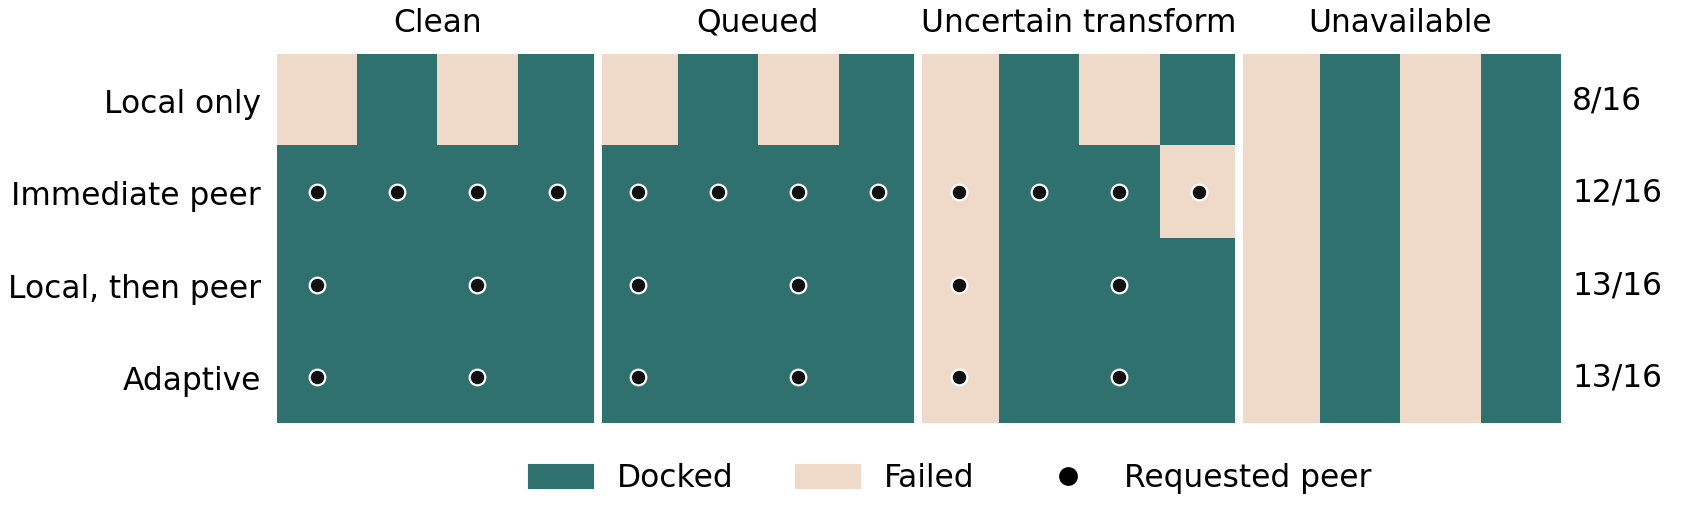
\includegraphics[width=\columnwidth]{figures/common-deadline-docking.png}
\caption{Within each service offer, each column represents the same starting scene across four policies. Adaptive and local-first calls led to the same docking outcomes.}
\end{figure}

\subsection{Requesting complementary skills in a delivery model}
A separate 2-D experiment, E1, repeated five fleet configurations in each of 96 rooms. The requested object and the recipient's initial information about location and grasp properties varied across rooms. The Tank could participate in a search stage; a station could supply an object-width measurement with simulated noise. Every condition used the same final virtual handover. Success required the requested object to be delivered within the 600\,s mission deadline. This model scores graspability using object width.

The fixed rule that enabled helpers according to assessed gaps delivered in 91/96 rooms. Always enabling both helpers delivered in 87/96. The paired outcomes were 86 deliveries by both, five by the gap rule alone, one by the always-on rule alone and four by neither (two-sided paired exact $p=0.219$). The station-only helper configuration also delivered in 91/96. The gap rule recorded a search stage with Tank available in 50 rooms and a station measurement stage in 48; the always-on condition recorded each stage in all 96. The search-stage flag identifies which robots were available. It cannot attribute the sighting to a particular camera. Across all paired rooms the gap rule used 29.40 fewer wall-clock seconds on average (median reduction 9.80\,s). Three always-on attempts reached the time limit. These capped mission times include host scheduling and use a different clock from the MuJoCo docking experiment.

\subsection{A three-robot message chain}
A tabletop arm viewed a coloured token with its wrist camera. The wheeled manipulator saw two docks and measured the one named by the token message. The tracked base received this pose and drove to the corresponding dock. Both colours appeared on each side of the target board across four prescribed layouts. The independent terminal check used the pose of the originally requested dock, including when the requested colour or the transmitted pose was deliberately changed. The team completed all four orders with the two correct messages. Suppressing or swapping either message yielded zero correct docks in each of the four interventions. This small test exercises routing, sensing and execution in one world. It does not estimate success on unseen arrangements or transfer to the physical fleet.

\begin{figure}[t]
\centering
\begin{tabular}{@{}cc@{}}
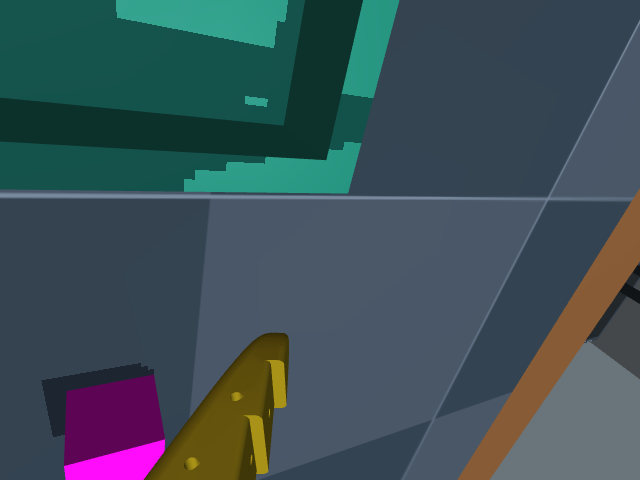
\includegraphics[width=.47\columnwidth]{figures/so101-order.png}&
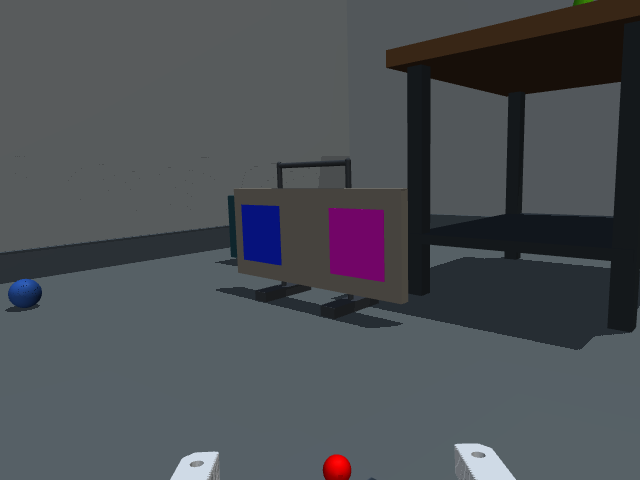
\includegraphics[width=.47\columnwidth]{figures/rosmaster-stations.png}\\
(a) Order at the tabletop & (b) Two candidate docks
\end{tabular}
\caption{Simultaneous roles in scene 868000. The wrist view supplied the colour and the mobile manipulator supplied metric position. The tracked robot received only the selected waypoint.}
\end{figure}

\section{Does the target measurement matter for grasping?}
A separate wheeled-arm experiment isolates localization from motor learning. A supervised ResNet-18 learned planar cube position from 1,024 simulated RGB images. The training labels use simulator geometry. At evaluation the arm takes a prescribed look, estimates the target from one image, then executes a rate-limited trajectory. Thirty-two training demonstrations provide 220-step, six-channel motor trajectories. Eight principal components fitted to these trajectories describe their variation. We used the LeRobot implementations of ACT \cite{act} and Diffusion Policy \cite{diffusion} to predict coefficients conditional on target position. This is a compressed trajectory adaptation of the two architectures. A thin-plate spline interpolates the demonstrations, and a geometric inverse-kinematics controller provides a second baseline. The experiment terminates on a stable hold in a carry pose. Placement and release require a different experiment.

\begin{table}[t]
\centering\caption{Successful simulated carry holds on the same 20 fresh starts per column. Each constant ablation uses the same training-set mean position.}
\begin{tabular}{lrr}\hline
Motor policy & Visual estimate & Constant target \\\hline
ACT & 15 & 2 \\
Diffusion & 18 & 2 \\
Thin-plate spline & 20 & 2 \\
Inverse kinematics & 18 & --- \\\hline
\end{tabular}
\end{table}

The first training seed used 1,000 ACT and 2,000 diffusion optimizer updates. Frozen development and fresh evaluation sets comprised eight and 20 scenes, respectively. Diffusion gained 16 fresh scenes over its own constant-target control and lost zero. A second, retrospective comparison matched initial arm angles, cube position and physics revision against 20 historical starts. Raw image-to-action ACT had produced six holds and raw diffusion one. The position-conditioned pipelines produced 19 and 20. Localization supervision, the deliberate look and the motor representation all changed together, so that comparison cannot isolate an architecture effect. The spline result also demonstrates that the extra neural motor model provided no observed advantage on the fresh set. A second replay applied the physical controller's native joint and gripper rate limits, command quantization and path checks, using simulated telemetry. On the same starts the spline, ACT and diffusion then held 17, 14 and 17 cubes. Sixty attempts used this command path; real actuators were disconnected from the replay.

In a separate moving-target experiment, the robot could return to its calibrated look pose before closure and generate a new trajectory. Half the starts received a 10\,mm lateral cube shift after six movement ticks. Fit, calibration and evaluation used 40, 24 and 32 distinct scenes. The endpoint was first stable carry within the original time budget. Reobservation on every start reached that endpoint in 28/32 against 21/32 without a second look (eight gains, one loss, exploratory exact paired $p=0.0391$). This differs from the fixed-horizon final retention endpoint. A visual failure probe missed all eleven baseline failures and made five false alarms. The template monitor made no calls. At the original strict visual check the first paired execution stopped before any pair was complete. A separately registered recovery used one archived RGB exposure at each common physical decision state, with the fitted model and thresholds unchanged. All 32 recovered pairs then executed their two terminal branches independently.

\section{Transfer and limits}
We retained the split between physical development recordings and sealed final evaluation recordings. On two archived physical development episodes, the first yielded no RGB frame within the required camera pose window. The second yielded one camera-pose match while wrist and gripper configuration differed from the trained observation posture. Neither episode had an independently checked mapping from RGB estimates to measured floor coordinates. The robot issued zero motor commands. Physical duplication of a simulated hold, or completion of a coordinated docking trial, remains to be measured.

Physical evaluation of a request rule requires the two platforms in a surveyed shared frame, verified camera mounts and stopping behaviour, paired initial placements, and an endpoint measured independently after the stop. The reported simulated outcomes and passive camera replays contribute zero measured physical docking or carry attempts to these comparisons.

\section*{Machine-generated evidence table}
Original and recovered comparisons use the same scene IDs. The earlier learned request rule had a three-second sensing allowance while the sequential rule could use six. Motor demonstrations, labelled camera images and independent evaluation scenes are counted separately.
% measured-results
\begin{table*}[t]
\centering\footnotesize
\caption{Evidence computed from archived simulator outcomes. Each denominator refers to its own registered scene bank.}
\begin{tabular}{@{}p{.24\textwidth}p{.71\textwidth}@{}}\hline
Comparison & Measured outcome \\\hline
Common-deadline peer docking & Local 8/16, immediate 12/16 (12 calls), local-first 13/16 (6 calls), adaptive 13/16 (6 calls). Adaptive gained 0 and lost 0 vs local-first. Mean utility difference +0.000875. \\
Recorded starts, raw ACT & Before 0/20, skill initialization 3/20, scratch 1/20. Baseline reset vectors were unavailable. \\
Fixed-look grasp & ACT 15/20 and Diffusion 18/20. Second optimizer seed on the same scenes gave 19 and 16. RBF 20, IK 18. \\
Native grasp admission & 29/128 eligible, 20 executed, 12 terminal holds. 9 eligible starts unexecuted. \\
Peer docking, original strict & Learned / local-first / always peer, each reported as success, calls and utility. 15/15, 13 calls, 0.86130 / 15/15, 8 calls, 0.89187 / 15/15, 15 calls, 0.84598. \\
Peer docking, including recovery & Learned / local-first / always peer, each reported as success, calls and utility. 16/16, 14 calls, 0.85959 / 16/16, 8 calls, 0.89545 / 16/16, 16 calls, 0.84523. \\
2D delivery, matched rooms & K0 63/96, K1 64/96, K2 91/96, K3 91/96, K5 87/96. K3 gained 2 and lost 2 against K2, gained 5 and lost 1 against K5. \\
Docking with common visual memory & Nav2 control law / PPO achieved 14 / 11 on 14 strict scenes, 16 / 12 on all 16 including RGB recovery. \\
Bounded motor correction & Terminal bilateral carry, original 31/32, fitted 29/32. 0 gained and 2 lost. Among 36 eligible of 160 assigned. \\
A second camera pose & Full target seen 11 to 17 on 32 assigned. Strict holds 4 to 4. \\
Learned RGB keypoint & Native unrestricted holds 29 to 27 on 48 fresh scenes. 8 gained and 10 lost. \\
Pre-closure reobservation & First stable carries 21 to 28 on 32 starts. The return gained 8 and lost 1. RGB probe missed 11/11 failures and raised 5 false alarms. Template tracker issued 0 alarms. \\
Archived human sequences & 5 full takes and 6 prefixes. Scratch 0/20, pretrained 0/20 terminal holds in MuJoCo. \\
\hline\end{tabular}
\end{table*}
% end-measured-results
\bibliographystyle{plainnat}
\bibliography{references}
\end{document}
